\chapter{Dinámica neuronal critica en el C. elegans}
\graphicspath{{figs/}}

\chapterquote{Quantum Mechanics is God's version of `Trust me.' }{Jorge Corona, 1982}

\label{titulo-cap-2}


%%%%%%%%%%%%%%%%%%%%%%%%%%%%%%%%%%%%%%%%%%%%%%%%%%%%%%%%%%%%%%%%%%%%%%%%
\section{Formulaci\'{o}n del problema}
\label{S:form-del-probl}

El problema de la medida se puede describir informalmente del siguiente modo 

\begin{enumerate}
\item  De acuerdo con la mec\'{a}nica cu\'{a}ntica cuando un sistema f\'{\i}sico, ya sea un conjunto de electrones orbitando en un \'{a}tomo, queda descrito por una funci\'{o}n de onda. Dicha funci\'{o}n de onda es un objeto matem\'{a}tico que supuestamente describe la m\'{a}xima informaci\'{o}n posible que contiene un estado puro.
\item  Si nadie externo al sistema ni dentro de \'{e}l observara o tratara de ver como est\'{a} el sistema, la mec\'{a}nica cu\'{a}ntica nos dir\'{\i}a que el estado del sistema evoluciona deterministamente. Es decir, que podr\'{\i}a ser perfectamente predecible hacia donde ir\'{a} el sistema.
\item  La funci\'{o}n de onda nos informa de cuales son los resultados posibles de una medida y sus probabilidades relativas, pero no nos dice qu\'{e} resultado concreto se obtendr\'{a} si un observador trata efectivamente de medir el sistema o averiguar algo sobre \'{e}l. De hecho, la medida sobre un sistema es un valor impredecible de entre los resultados posibles.

Eso plantea un problema serio, si las personas, los cient\'{\i}ficos u observadores son tambi\'{e}n objetos f\'{\i}sicos como cualquier otro, deber\'{\i}a haber alguna forma determinista de predecir como tras juntar el sistema en estudio con el aparato de medida, finalmente llegamos a un resultado determinista. Pero el postulado de que una medici\'{o}n destruye la ``coherencia'' de un estado inobservado e inevitablemente tras la medida se queda en un estado mezcla impredecible parece que s\'{o}lo nos deja 3 salidas (ver notas a continuaci\'{o}n):
\begin{enumerate}
\item O bien pasamos a entender el proceso de decoherencia por lo cual un sistema pasa de tener un estado puro que evoluciona predeciblemente a tener un estado mezcla o impredecible (ver teor\'{\i}a del caos)
\item  O bien admitimos que existen unos objetos no-f\'{\i}sicos llamados ``conciencia'' que no est\'{a}n sujetos a las leyes de la mec\'{a}nica cu\'{a}ntica y que nos resuelven el problema.
\item  O tratamos de inventar cualquier hip\'{o}tesis ex\'{o}tica que nos haga compatibilizar como por un lado deber\'{\i}amos estar observando tras una medida un estado no fijado por el estado inicial y por otro lado que el estado del universo en su conjunto evoluciona de forma determinista.
\end{enumerate}
\textquote{Prueba \textquote{prueba}}
El enunciado anterior ``una medici\'{o}n destruye la 'coherencia' de un estado inobservado e inevitablemente tras la medida se queda en un estado mezcla impredecible parece que s\'{o}lo nos deja 3 salidas'' es demasiado arriesgado y no probado. Si partimos de que las entidades fundamentales que constituyen la materia, precisamente, y al contrario de lo que deduce (B) no tienen consciencia de s\'{\i} mismas, y sin preferencia alguna por el determinismo o el caos absoluto, s\'{o}lo pueden encontrar el equilibrio comport\'{a}ndose seg\'{u}n leyes de probabilidad o lo que es lo mismo por leyes de ``caos determinado''. En la pr\'{a}ctica cualquier defensa o negaci\'{o}n de la teor\'{\i}a cu\'{a}ntica no responde a razonamientos matem\'{a}ticos deductivos sino a impresiones o sugestiones con origen en axiomas filos\'{o}ficos totalmente arbitrarios. Notar que p.ej, la palabra ``equilibrio'' en este p\'{a}rrafo puede o no tener sentido y el valor de realidad que se conceda al mismo no est\'{a} sujeto a demostraci\'{o}n matem\'{a}tica alguna.
\end{enumerate}


\section{Interpretaciones}
\label{S:interpretaciones}

Com\'{u}nmente existen diversas interpretaciones de la mec\'{a}nica cu\'{a}ntica, cada una de las cuales en general afronta el problema de la medida de manera diferente. De hecho si el problema de la medida estuviera totalmente no existir\'{\i}an algunas de las interpretaciones rivales. En cierto modo la existencia de diferentes interpretaciones refleja que no existe un consenso sobre como plantear precisamente el problema de la medida. Algunas de las interpretaciones m\'{a}s ampliamente conocidas son las siguientes:

\begin{enumerate}
\item Interpretaci\'{o}n estad\'{\i}stica, en la que se supone un estado cu\'{a}ntico describe una
  regularidad estad\'{\i}stica, siendo explicables los diferentes resultados de la medida de un
  observable atribuibles a factores estoc\'{a}sticos o fluctuaciones debidas al entorno y no
  observables. La electrodin\'{a}mica estad\'{\i}stica es una teor\'{\i}a de los electrones en que el
  comportamiento cu\'{a}ntico, aparentemente aleatorio, de los electrones de un sistema es
  atribuible a las fluctuaciones del campo electromagn\'{e}tico debido al resto de electrones
  del universo.
  
  \autoref{fig:1}
  
\begin{figure}[ht]
\centering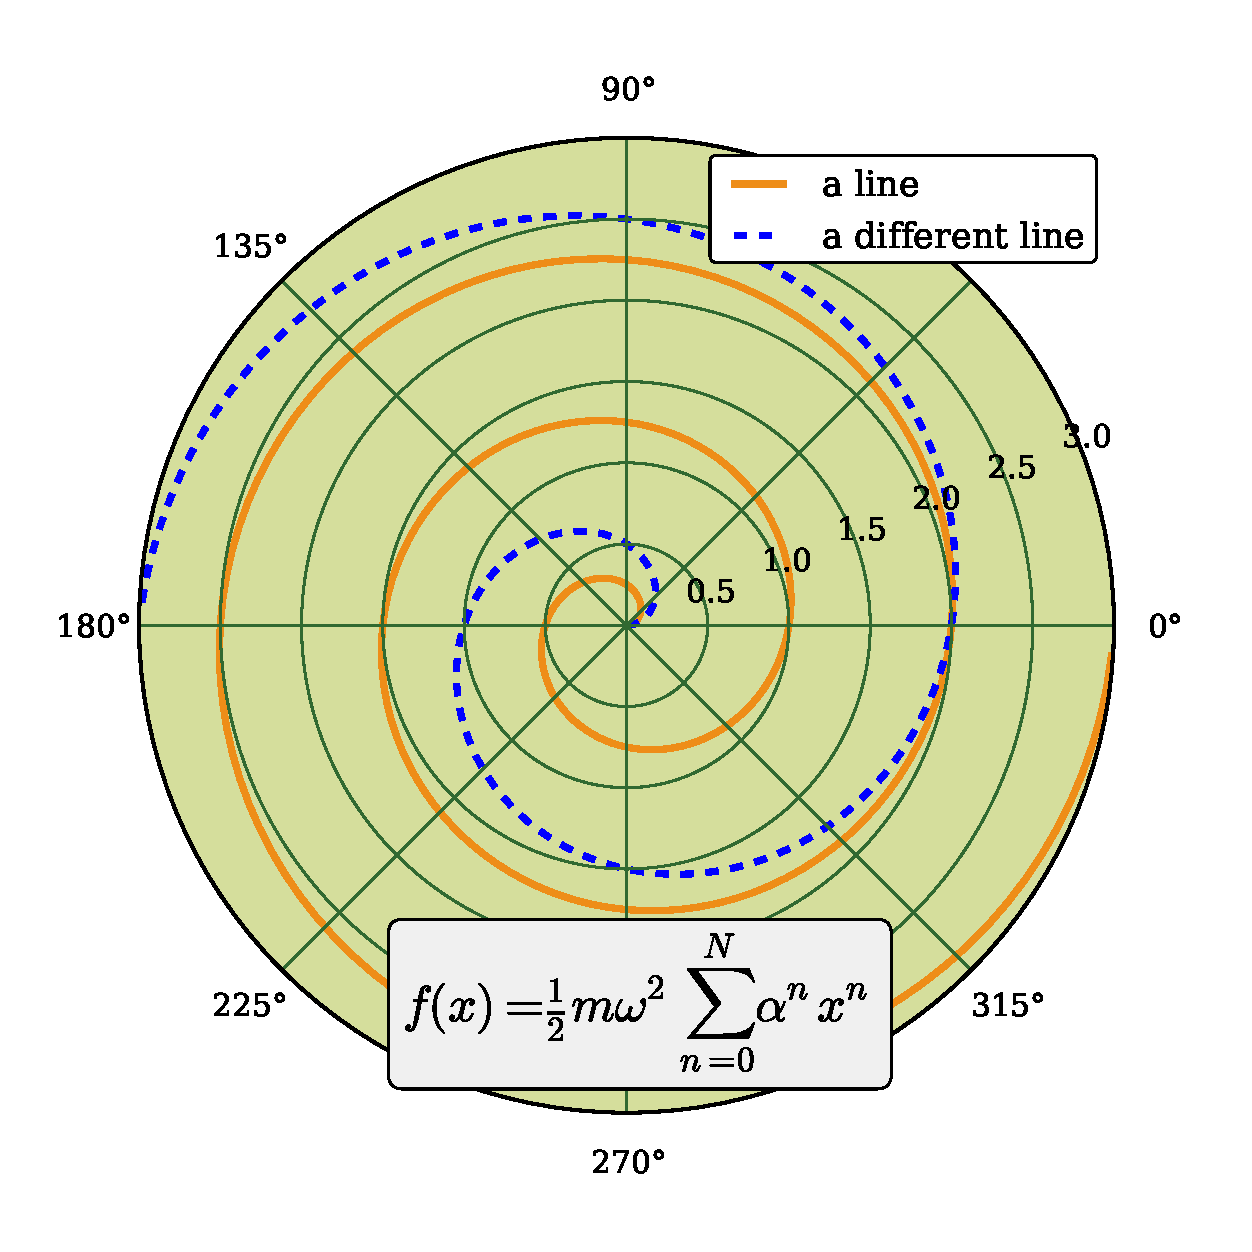
\includegraphics[width=\imsize]{cap2_f1}
\caption[La figura muestra algunas curvas m\'{a}s o menos lindas]{La figura muestra algunas curvas m\'{a}s o menos lindas. El gr\'{a}fico est\'{a} en coordenadas porlares como se muestra en la }
\end{figure}\label{fig:1}

\autoref{tabla:1}

\begin{table}
\begin{tabular}{@{}llr@{}} \toprule
	\multicolumn{2}{c}{Item} \\ \cmidrule(r){1-2}
	Animal & Description & Price (\$)\\ \midrule
	Gnat & per gram & 13.65 \\
	& each & 0.01 \\
	Gnu & stuffed & 92.50 \\
	Emu & stuffed & 33.33 \\
	Armadillo & frozen & 8.99 \\ \bottomrule
\end{tabular}
\end{table}\label{tabla:1}
\item Interpretaci\'{o}n de Copenhague, es la interpretaci\'{o}n probablemente m\'{a}s com\'{u}n y a la
  que se han adherido la mayor\'{\i}a de manuales de mec\'{a}nica cu\'{a}ntica tradicionalmente. Debida
  inicialmente a Niels Bohr y el grupo de f\'{\i}sicos que trabajaba con \'{e}l en Copenhague hacia
  1927. Se asume el principio de incertidumbre y el principio de complementariedad de las
  descripciones ondulatoria y corpuscular.
\item Interpretaci\'{o}n participatoria del principio antr\'{o}pico.
\item Interpretaci\'{o}n de historias consistentes.
\item Teor\'{\i}as de colapso objetivo.De acuerdo con estas teor\'{\i}as, la superposiciones de
  estados se destruyen aunque no se produzca observaci\'{o}n, difiriendo las teor\'{\i}as en qu\'{e}
  magnitud f\'{\i}sica es la que provoca la destrucci\'{o}n (tiempo, gravitaci\'{o}n,temperatura,
  t\'{e}rminos no lineales en el operador de evoluci\'{o}n...). Esa destrucci\'{o}n es lo que evita
  las ramas que aparecen en la teor\'{\i}a de los multi-universos o universos paralelos . La
  palabra "objetivo" procede de que en esta interpretaci\'{o}n tanto la funci\'{o}n de onda como
  el colapso de la misma son "reales", en el sentido ontol\'{o}gico.En la interpretaci\'{o}n de
  los muchos-mundos, el collapso no es objetivo, y en la de Copenhague es una hip\'{o}tesis
  ad-hoc.

  \begin{itemize}
  \item Interpretaci\'{o}n multiverso.
  \item Decoherencia por el entorno
  \item Interpretaci\'{o}n de Bohm
  \item Interpretaci\'{o}n Madhyamika
  \end{itemize}
\end{enumerate}

En la primera ecuaci\'{o}n
\begin{equation}
\phi_{1}(z)=A_{1}e^{ik_{1}z}+B_{1}e^{-ik_{1}z}.
\end{equation}

En la segunda ecuaci\'{o}n:
\begin{equation}
\phi_{2}(z)=A_{2}e^{ik_{2}z}+B_{2}e^{-ik_{2}z}.
\end{equation}

La soluci\'{o}n de la tercera ecuaci\'{o}n se puede obtener a partir de la
soluci\'{o}n en la primera ecuaci\'{o}n aplicando 
\begin{equation}
\phi_{3}(z)=e^{iKd}(A_{1}e^{ik_{1}(z-l)}+B_{1}e^{-ik_{1}(z-l)}).
\end{equation}

\chapter{otr}
\label{C:otr}

\section{Secci\'{o}n 1}
\label{S:seccion-1}

\section{otra}
\label{S:otra}

\section{una}
\label{S:una}

\section{dos}
\label{S:dos}

\section{tres}
\label{S:tres}

\chapter{cuatro}
\label{C:cuatro}

\section{una}
\label{S:una-1}

\section{otra mas}
\label{S:otra-mas}


%%% Local Variables: 
%%% mode: latex
%%% TeX-master: "template"
%%% End: 
